\section{Anomaly detection}\label{sec:anomaly}
Raw values would flag every Arctic or desert capital simply for being itself. Anomalies are therefore defined
relative to each city's own climate: temperature is standardised against the city-and-month mean, and the
other variables against the city mean. Four complementary detectors are used.
\begin{enumerate}
  \item \textbf{Isolation Forest} (300 trees, 1\,\% contamination) on ten locally standardised variables.
        It flags 1\,668 observations.
  \item \textbf{Local Outlier Factor} ($k=35$) on a 60\,000-row sample.
  \item \textbf{Temporal robust $z$-score}: temperature against a centred 15-day rolling median, scaled by the
        city's MAD, with $|z|>3.5$. This flags 2.6\,\% of observations, mostly sudden cold snaps or heat spikes.
  \item \textbf{Batch-level detector} (Figure~\ref{fig:batch}): days on which most cities deviate at once.
        This is a data-pipeline failure, not weather.
\end{enumerate}

Isolation Forest anomalies are driven mainly by extreme precipitation, low visibility and humidity
(Figure~\ref{fig:anomdrivers}): storms and fog events. Isolation Forest and LOF overlap only moderately
(Jaccard $\approx 0.11$). The global method looks for rare \emph{combinations}, while LOF finds sparse
neighbourhoods. About 18\,\% of Isolation Forest anomalies are also temporal anomalies, and about 19\,\% contain
a value capped during cleaning. The multivariate view therefore adds information beyond univariate fences.

\begin{figure}[H]\centering
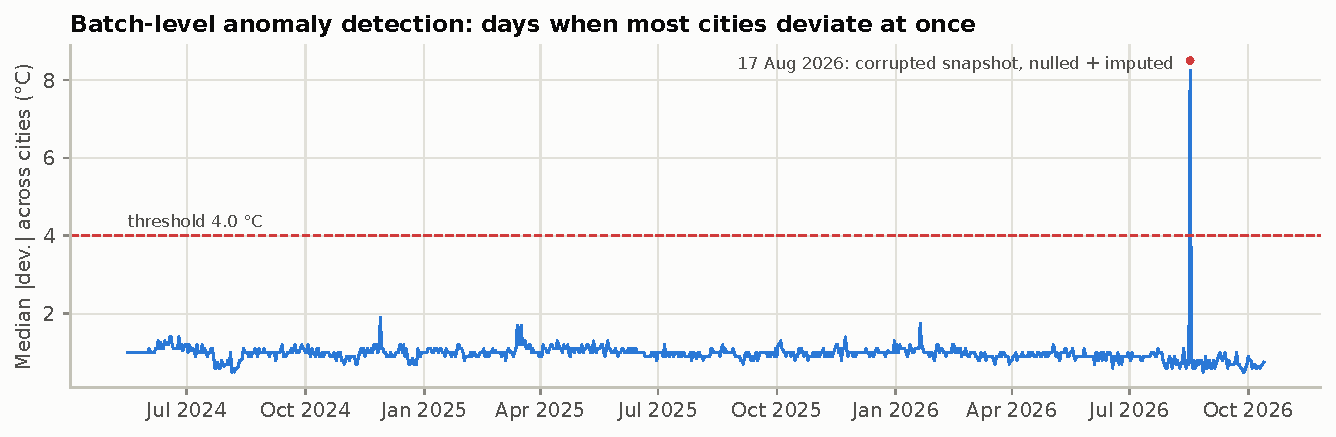
\includegraphics[width=0.9\linewidth]{anomaly/batch_corruption_detector}
\caption{Batch-level detector: the 17~Aug~2026 snapshot is corrupted and was nulled and imputed during cleaning.}\label{fig:batch}
\end{figure}
\begin{figure}[H]\centering
\begin{subfigure}{0.49\linewidth}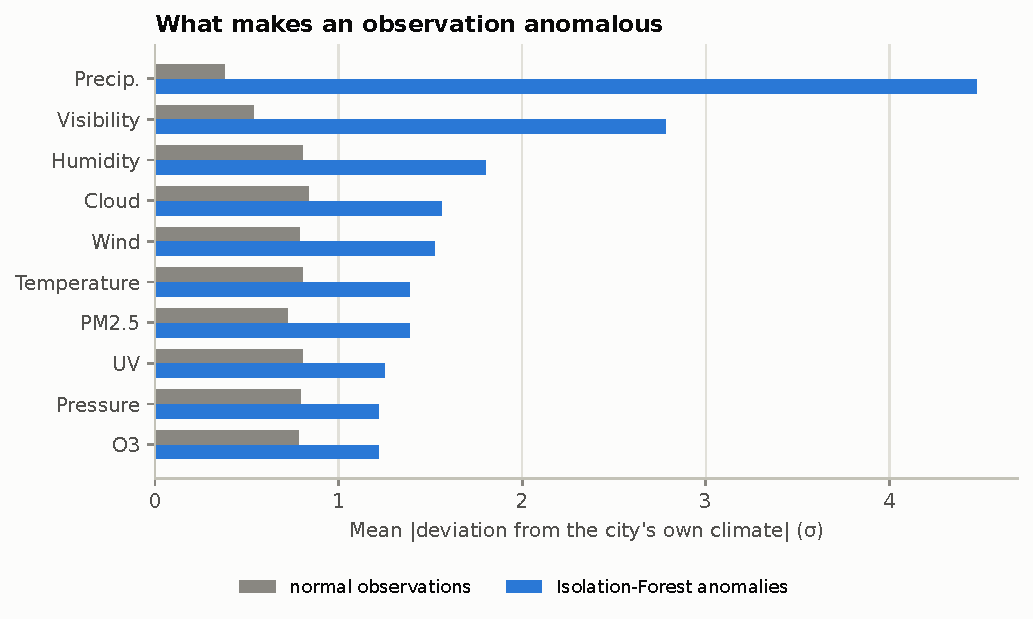
\includegraphics[width=\linewidth]{anomaly/anomaly_drivers}\caption{Drivers}\label{fig:anomdrivers}\end{subfigure}
\begin{subfigure}{0.49\linewidth}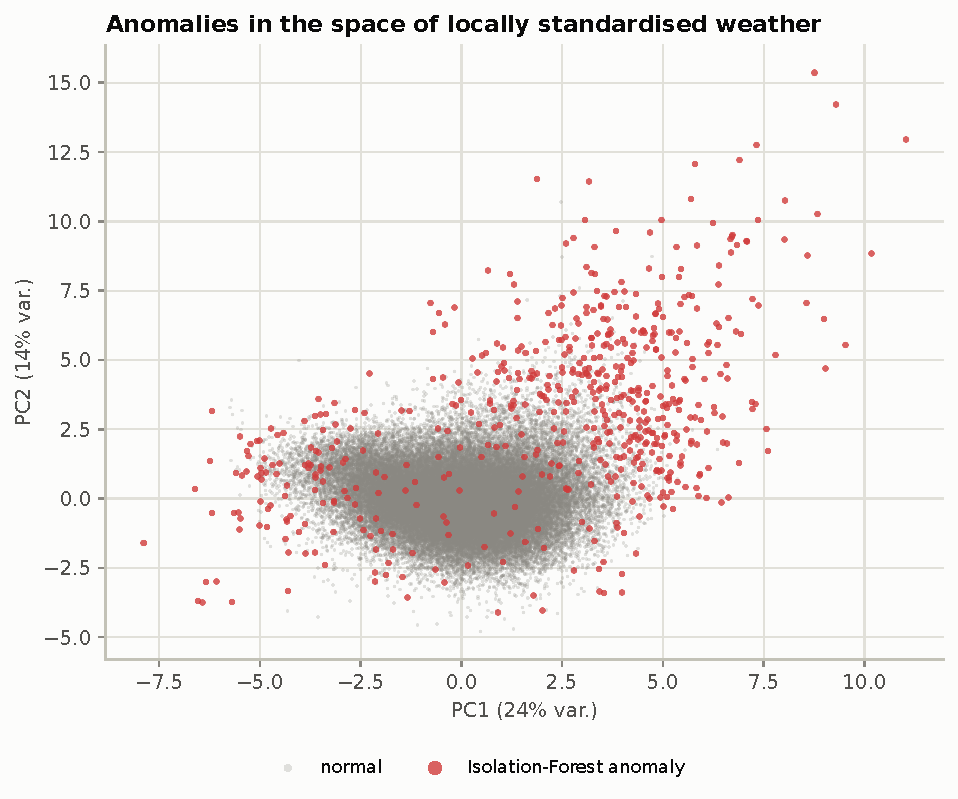
\includegraphics[width=\linewidth]{anomaly/anomaly_pca}\caption{PCA projection}\end{subfigure}
\caption{What makes an observation anomalous, and where anomalies sit in the locally standardised weather space.}
\end{figure}
\begin{figure}[H]\centering
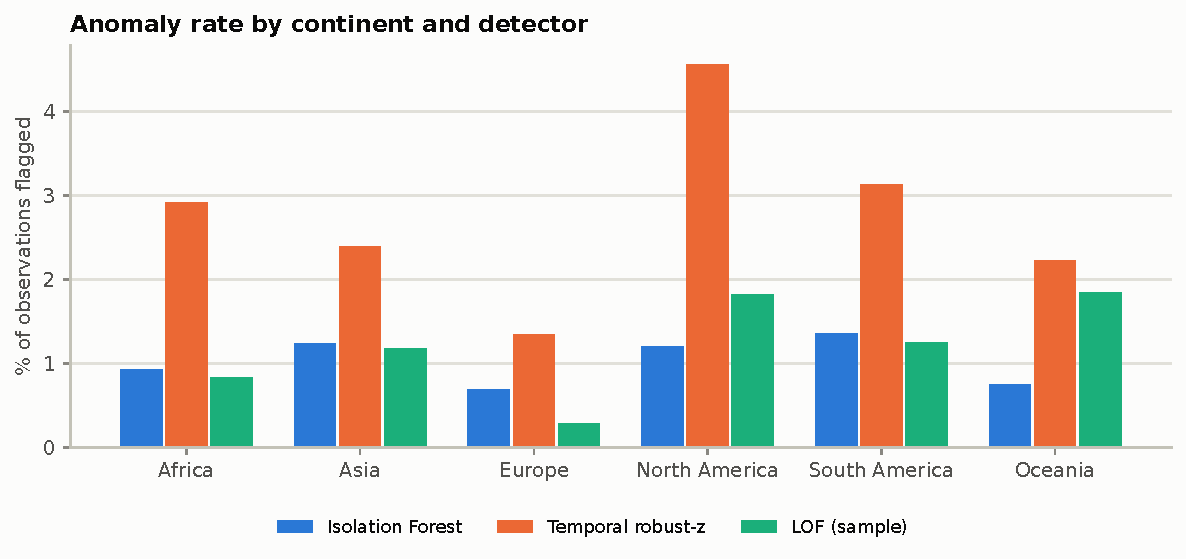
\includegraphics[width=0.85\linewidth]{anomaly/anomaly_rate_by_continent}
\caption{Anomaly rate by continent and detector.}
\end{figure}
\begin{figure}[H]\centering
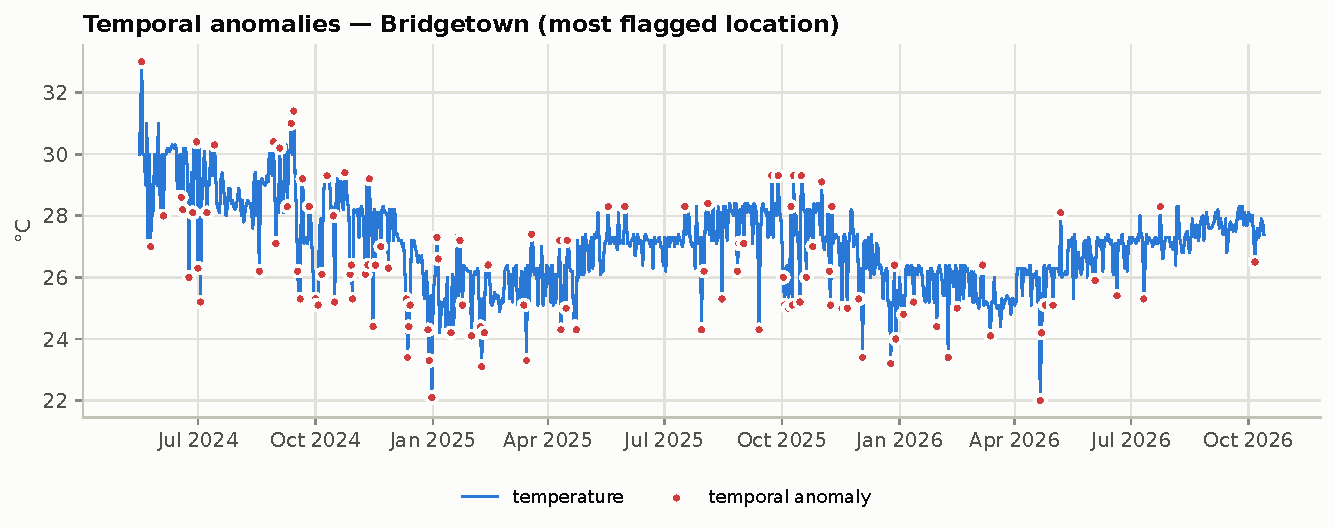
\includegraphics[width=0.9\linewidth]{anomaly/city_temporal_anomalies}
\caption{Temporal anomalies for the most-flagged capital.}
\end{figure}
\begin{figure}[H]\centering
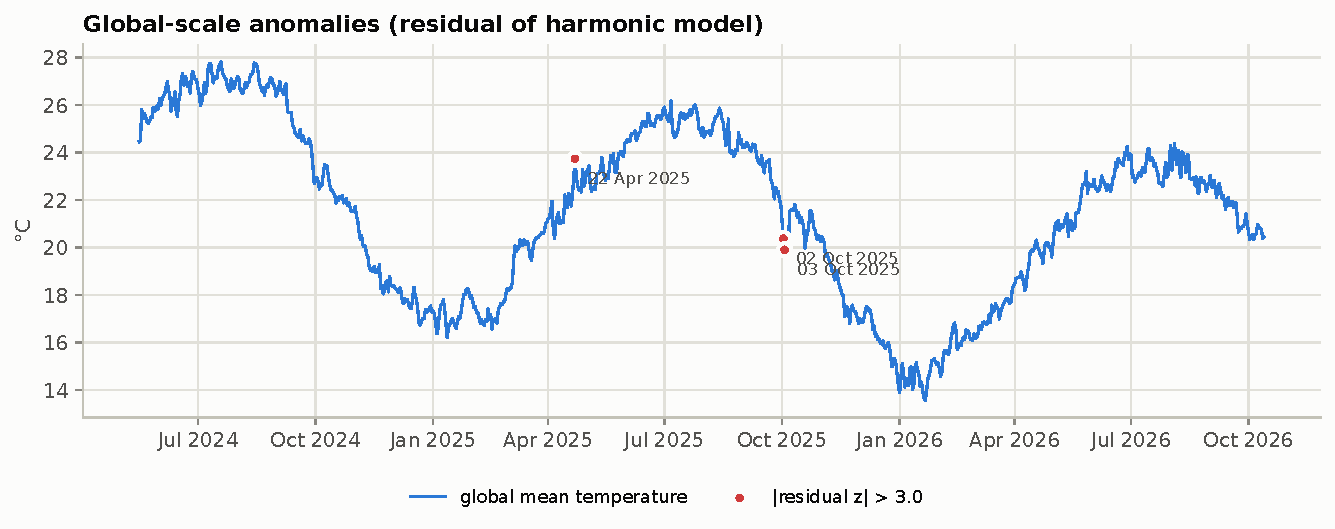
\includegraphics[width=0.9\linewidth]{anomaly/global_anomalies}
\caption{Remaining global-scale anomalies after cleaning ($|z|>3$ on the residual of the harmonic model).}
\end{figure}
\tbl{top_anomalies.tex}
